\documentclass{beamer}
\usepackage{beamerthemesplit}
\usetheme{SPbGU}
%{CambridgeUS}
% Выпишем часть возможных стилей, некоторые из них могут содержать
% дополнительные опции
% Darmstadt, Ilmenau, CambridgeUS, default, Bergen, Madrid, AnnArbor,Pittsburg, Rochester,
% Antiles, Montpellier, Berkley, Berlin
\usepackage{pdfpages}
\usepackage{amsmath}
\usepackage{cmap} % for serchable pdf's
\usepackage[T2A]{fontenc} 
\usepackage[utf8]{inputenc}
\usepackage[english,russian]{babel}
%\uselanguage{russian}\languagepath{russian}
\usepackage{indentfirst}
\usepackage{amsmath}
%\usepackage{dot2texi}
\usepackage{tikz}
\usepackage{multirow}


\usepackage[noend]{algpseudocode}
\usepackage{algorithm}
\usepackage{algorithmicx}
%\usepackage{mathspec}

\usetikzlibrary{shapes,arrows}
\usepackage{fancyvrb}

\newtheorem{rutheorem}{Теорема}
\newtheorem{ruproof}{Доказательство}
\newtheorem{rudefinition}{Определение}
\newtheorem{rulemma}{Лемма}

% Если у вас есть логотип вашей кафедры, факультета или университета, то
% его можно включить в презентацию.

%\usefoottemplate{\vbox{}}%  \tinycolouredline{structure!25}% {\color{white}\textbf{\insertshortauthor\hfill% \insertshortinstitute}}% \tinycolouredline{structure}% {\color{white}\textbf{\insertshorttitle}\hfill}% }}

%\logo{
\includegraphics[width=1cm]{SPbGU_Logo.png}}

%[GLR-анализатор]
\title[]{Cинтаксический анализ динамически формируемых строковых выражений}
%\subtitle[студроект]{Студенческий проект}
\institute[СПбГУ]{
Санкт-Петербургский государственный университет \\
Математико-Механический факультет \\
Кафедра системного программирования }
%[Лукичёв А.С. Григорьев С.В.]


\author[Григорьев Семён]{Григорьев Семён Вячеславович \\
  \and  
  {\bfseries Научный руководитель:} кандидат физико-математических наук, доцент Д.В. Кознов \\ 
%  \and
%  {\bfseries Рецензент:} д.ф.-м.н., проф. Б.К. Мартыненко  
}

\date{2015г.}

\definecolor{orange}{RGB}{179,36,31}

\begin{document}
{

\begin{frame}
\begin{center}
{
\includegraphics[width=1cm]{SPbGU_Logo.png}}
\end{center}
\titlepage
\end{frame}
}

\begin{frame}[fragile]
    \transwipe[direction=90]
    \frametitle{Динамически формируемые строковые выражения: пример}
    \begin{itemize}
        \item Встроенный SQL
\begin{Verbatim}[commandchars=\\\{\}]
\textcolor{blue}{let} p cond fldLst =
    \textcolor{blue}{let mutable} flds = \textcolor{orange}{"id"}
    \textcolor{blue}{for} fld \textcolor{blue}{in} fldLst \textcolor{blue}{do}
        flds <- flds + \textcolor{orange}{", "} + fld 
    \textcolor{blue}{let} tbl = \textcolor{blue}{if} cond \textcolor{blue}{then} \textcolor{orange}{"table1"} \textcolor{blue}{else} \textcolor{orange}{"table2"}    
    \underline{execute} (\textcolor{orange}{"SELECT"} + flds + \textcolor{orange}{"FROM"} + tbl)
\end{Verbatim}
        \item JavaScript в Java
\begin{Verbatim}[commandchars=\\\{\}]
\textcolor{blue}{String} script =
    \textcolor{orange}{"function hello(name) { print(’Hello, ’ + name); }"};
engine.eval(script);
\textcolor{blue}{Invocable} inv = (\textcolor{blue}{Invocable}) engine;
inv.invokeFunction(\textcolor{orange}{"hello"}, \textcolor{orange}{"Scripting!!!"} );
\end{Verbatim}
    \end{itemize}

\end{frame}

\begin{frame}
    \transwipe[direction=90]
    \frametitle{Динамически формируемые строковые выражения: проблемы}
    \begin{itemize}
        \item Значение выражения -- код на некотором языке и его нужно соответствующим образом поддерживать и обрабатывать
        \item Однако для стандартных инструментов это просто строки
        \begin{itemize}
            \item Ошибки в динамически формируемых выражениях обнаруживаются лишь во время выполнения
            \item Нет поддержки в средах разработки
            \item Затруднён реинжиниринг ПО, разработанного с использованием встроенных языков                
        \end{itemize}
        \item Существует множество различных языков и задач
    \end{itemize}
\end{frame}

\begin{frame}
    \transwipe[direction=90]
    \frametitle{Обзор}
    \begin{itemize}
        \item Построение аппроксимации $L_R \rightarrow $ \ проверка включения $L_{R} \subseteq L(G)$, $G$ -- КС грамматика референсного языка 
        \begin{itemize}
            \item JSA, PHPSA
        \end{itemize}
        \item Alvor -- построение регулярной аппроксимации  $ \rightarrow $ \ лексический анализ $ \rightarrow $ \ синтаксический анализ
        \item Kyung-Goo Doh -- data-flow уравнения + LALR(1) анализ + абстрактная интерпретация стеков + атрибутные грамматики
        \item Для работы с сематникой нужно иметь лес вывода -- множество деревьев для всех $\omega \in L_R$ выводимых в G
    \end{itemize}
\end{frame}

\begin{frame}
    \transwipe[direction=90]
    \frametitle{Цели и задачи работы}
    \begin{itemize}
        \item Создать подход к статическому синтаксическому анализу динамически формируемых выражений, позволяющего обрабатывать произвольную регулярную аппроксимацию без потери точности.
        \begin{itemize}
            \item Обработка регулярной аппроксимации
            \item Построение леса вывода
        \end{itemize}
        \item Разработать технологию для создания инструментов статического анализа встроенных текстовых языков, реализующую данный алгоритм.
    \end{itemize}
\end{frame}

\begin{frame}
    \transwipe[direction=90]
    \frametitle{Положения, выносимые на защиту}
        \begin{itemize}
            \item Разработан алгоритм синтаксического анализа динамически формируемых выражений, позволяющий обрабатывать произвольную регулярную аппроксимацию множества значений выражения в точке выполнения, реализующий эффективное управление стеком и гарантирующий конечность представления леса вывода. Доказана завершаемость и корректность предложенного алгоритма.
            \item Создана архитектура инструментария для разработки программных средств синтаксического анализа динамически формируемых строковых выражений.
            \item Разработана методика анализа динамически формируемых строковых выражений в проектах по реинжинирингу информационных систем.  
        \end{itemize}
\end{frame}

\begin{frame}
    \transwipe[direction=90]
    \frametitle{Научная новизна}
    \begin{itemize}
        \item Предложенный алгоритм предназначен для синтаксического анализа динамически формируемых выражений и построения компактной структуры данных, содержащей для всех корректных значений выражения их деревья вывода.
        \item Предложена архитектура инструментального средства, позволяющего упростить создание новых инструментов для анализа динамически формируемых выражений на любых языках программирования.
    \end{itemize}
\end{frame}

\begin{frame}
    \transwipe[direction=90]
    \frametitle{Архитектура: цели и задачи}
    \begin{itemize}
        \item Упростить создание инструментов анализа динамически формируемых выражений
        \item Необходим набор готовых компонентов, генераторы лексических и синтаксических анализаторов
    \end{itemize}
\end{frame}

\begin{frame}
    \transwipe[direction=90]
    \frametitle{Архитектура: процесс анализа}
    \begin{center}
        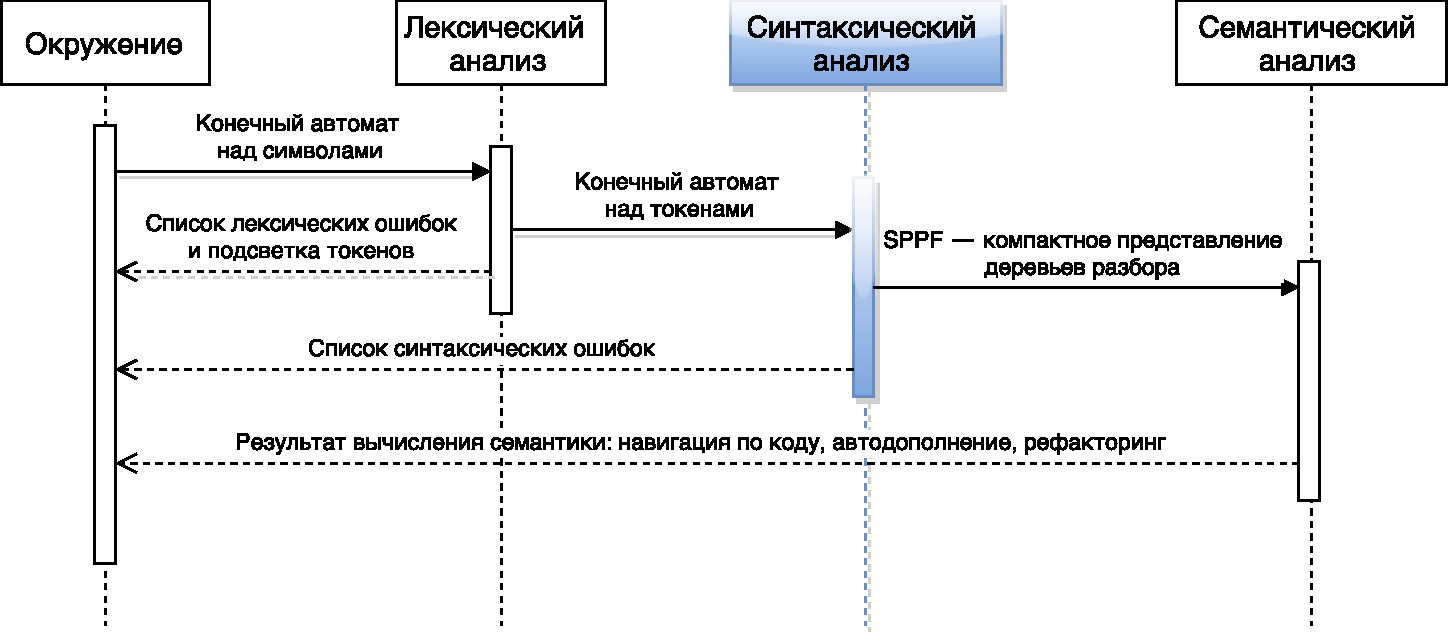
\includegraphics[width=300pt]{pictures/Seq.pdf}
    \end{center}
\end{frame}

\begin{frame}
    \transwipe[direction=90]
    \frametitle{Архитектура: инструментарий}
    \begin{center}
        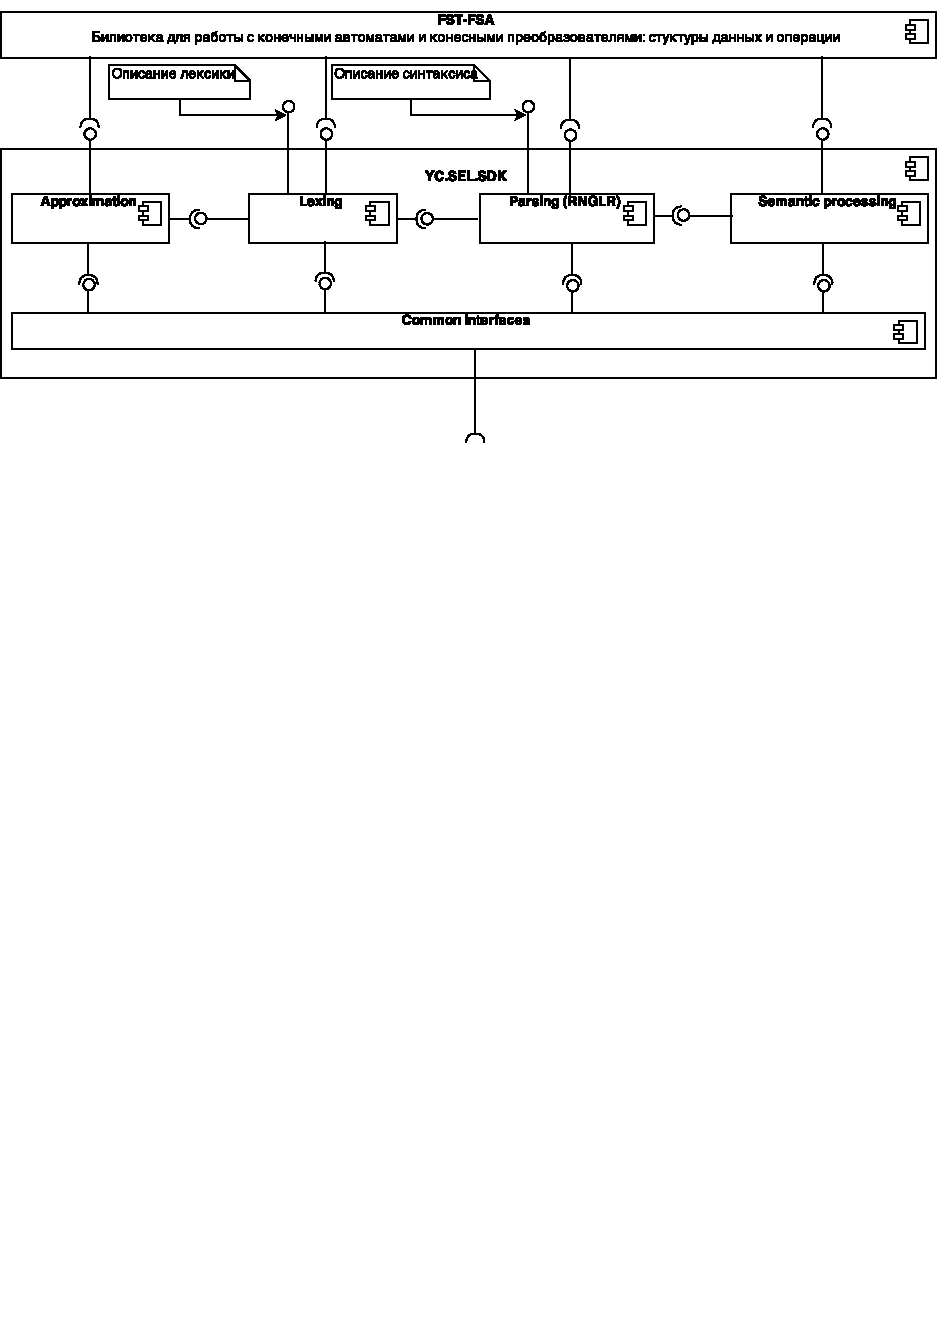
\includegraphics[width=300pt]{pictures/Components.pdf}
    \end{center}
\end{frame}

\begin{frame}[fragile]
    \transwipe[direction=90]
    \frametitle{Аппроксимация и лексический анализ}    
    \begin{itemize}    
        \item Используется регулярное приближение сверху множества значений выражения  
        \item Для лексического анализа используются конечные преобразователи
    \end{itemize}

\begin{center}
    \begin{tabular}{p{6cm}|p{6cm}}
    \begin{minipage}{3in}

        \begin{Verbatim}[commandchars=\\\{\}]
\textcolor{blue}{string} expr = \textcolor{orange}{"()"}
\textcolor{blue}{while} (cond) \textcolor{blue}{do} 
    expr := \textcolor{orange}{"("} + expr + \textcolor{orange}{")"}
\underline{evaluate(expr)}  
        \end{Verbatim}
    \end{minipage}
&
\\      
Аппроксимация: & Результат лексического анализа:
\\
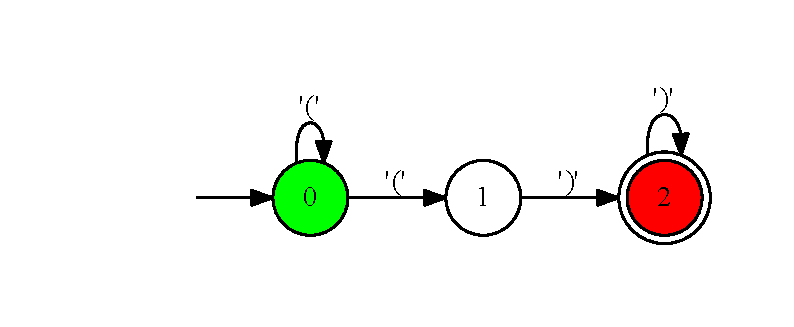
\includegraphics[width=150pt]{pictures/in3_appr.pdf}
&
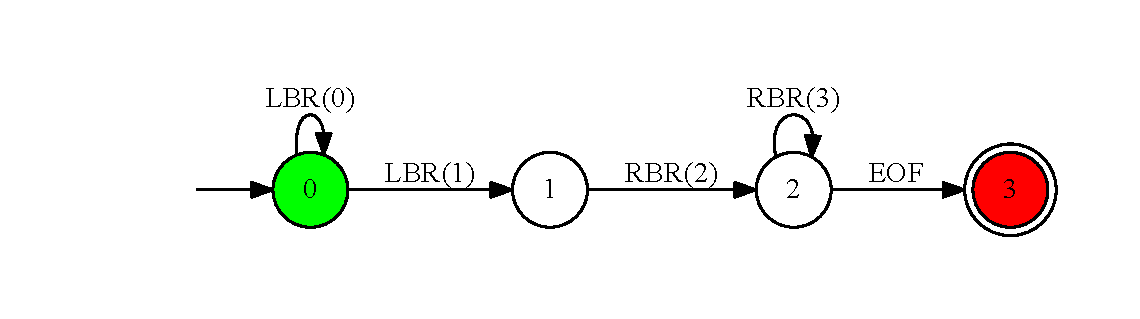
\includegraphics[width=160pt]{pictures/in3.pdf}

    \end{tabular}
\end{center}
\end{frame}

\begin{frame}
    \transwipe[direction=90]
    \frametitle{Синтаксический анализ: постановка задачи}
    \begin{itemize}    
        \item $G=\langle N,\Sigma, P,S\rangle$ -- однозначная КС грамматика
        \item $R$ -- регулярное множество над алфавитом ${\Sigma}^{'} \subseteq \Sigma $
        \item $AST(t,\omega,G)$ -- является ли $t$ деревом вывода $\omega$ в грамматике $G$
    \end{itemize}
    Необходимо построить алгоритм $\mathbb{P}$ такой что
    $(\forall \omega \in R) (\omega \in L(G) \Rightarrow (\exists t \in \mathbb{P}(R,G))AST(t, \omega, G))$
    $\land (\forall t \in \mathbb{P}(R,G))(\exists \omega \in R)AST(t,\omega,G)$
\end{frame}

\begin{frame}
    \transwipe[direction=90]
    \frametitle{Синтакический анализ: идеи алгоритма}
    \begin{itemize}         
        \item Основан на RNGLR алгоритме
        \begin{itemize}         
           \item Обрабатывает произвольные КС грамматики (в том числе неоднозначные)
           \item Основные операции: {\bfseries{\textit{push}}} -- композиция переноса и goto; {\bfseries{\textit{reduce}}} -- свёртка
           \item Использует компактное представление множества стеков ({\bfseries GSS}) и компактное представление леса разбора ({\bfseries SPPF})
        \end{itemize}
        \item Замена линейного входного потока на граф конечного автомата
        \item Обход графа и последовательное построение GSS по аналогии с RNGLR
            \begin{itemize}         
                \item Для каждой вершины входного графа вычисляется множество возможных вершин GSS -- состояний LR-анализатора
            \end{itemize}
        \item Построение SPPF как в RNGLR
        \item Использование очереди $\mathcal Q$ для задания последовательности обхода вершин
            \begin{itemize}         
                \item Вершина добавляется в $\mathcal Q$ если добавляется новое ребро в GSS с концом в этой вершине
            \end{itemize}
    \end{itemize}
\end{frame}

\begin{frame}
    \transwipe[direction=90]
    \frametitle{Синтакический анализ: идеи алгоритма}
    \begin{itemize}         
         \item {\bfseries{\textit{Свёртка}}} -- путь в GSS (путь в графе)
         \item {\bfseries{\textit{Проходящая свёртка}}} -- тройка $(startV, N, l)$, представляющая информацию о свёртке, проходившей через данную GSS вершину
         \begin{itemize}         
                \item $startV$ -- начало пути
        \item $N$ -- продукция, по которой нужно произвести свёртку
        \item $l$ -- длинна оставшегося пути
         \end{itemize}
    \end{itemize}
\end{frame}

\begin{frame}
    \transwipe[direction=90]
    \frametitle{Синтакический анализ: идеи алгоритма}
    \begin{itemize}
    \item Вершины GSS связываются с позицией во входном потоке, аналогично RNGLR
        \begin{itemize}
        \item Позиция -- состояние входного конечного автомата        
        \end{itemize}    
    \item Строится вспомогательная структура данных (\emph{внутренний граф}) -- копия входного автомата с вершинами, хранящими дополнительную информацию
        \begin{itemize}
        \item \emph{processed}: вершины GSS, для который все свёртки выполнены 
%   This set aggregates all GSS vertices, associated with inner graph vertex.
        \item \emph{unprocessed}: вершины GSS, для которых требуется выполнение переноса токенов
%   GSS vertices, for which all the pushes are to be processed. This set is analogous to $\mathcal{Q}$ of original RNGLR.
        \item \emph{reductions}: очередь свёрток, которые необхоимо выполнить
  % a queue, which is analogous to $\mathcal{R}$ of original RNGLR:  all reductions to be processed.
        \item \emph{passingReductionsToHandle}: набор пар из вершины и ребра GSS для выполнения проходящих свёрток
  %pairs of GSS vertex and GSS edge to apply  passing reductions along them.
        \end{itemize}
    \end{itemize}
\end{frame}

\begin{frame}[fragile] 
    \transwipe[direction=90]
    \frametitle{Алгоритм синтаксического анализа: основной цикл}
\begin{algorithmic}[1]
\Function{parse}{$grammar, automaton$}
  \State{$inputGraph \gets$ construct inner graph representation of $automaton$}
  \State{$parserSource \gets$ generate RNGLR parser tables for $grammar$}
  \State{\Call{addVertex}{$inputGraph.startVertex, startState$}}
  \State{$\mathcal{Q}.Enqueue(inputGraph.startVertex)$}
  \While{$Q$ is not empty}
    \State{$v \gets \mathcal{Q}.Dequeue()$}
    \State{\Call{makeReductions}{$v$}}
    \State{\Call{push}{$v$}}
    \State{\Call{applyPassingReductions}{$v$}}
  \EndWhile
  \If{$v_f.level = q_f$ and $v_f.state$ is accepting} {report success}
  \Else { report failure}
  \EndIf
\EndFunction
\end{algorithmic}
\end{frame}

\begin{frame}
    \transwipe[direction=90]
    \frametitle{Алгоритм: завершаемость}
    \begin{rutheorem}
             Алгоритм завершается для любой однозначной КС грамматики $G$ и любого КА без $\varepsilon-$переходов.
    \end{rutheorem}

    \begin{ruproof}
       Каждая вершина внутреннего графа содержит не более чем $N$ вершин GSS, где $N$ -- количество состояний LR-анализатора. Таким образом, всего может быть создано не более $N\times n$ вершин GSS, где $n$
       -- количество вершин во внутреннем графе. Так как GSS не содержит кратных дуг, то количество дуг в GSS не более, чем $O((N\times n)^2)$. Алгоритм извлекает одну вершину из  $\mathcal Q$ на каждой итерации.
       При этом вершины добавляются в $\mathcal Q$ только если добавляется новое ребро в GSS. Так как количество рёбер в GSS конечно, то алгоритм завершается.
       \qed
    \end{ruproof}

\end{frame}

\begin{frame}
    \transwipe[direction=90]
    \frametitle{Алгоритм: корректность. Определения}
    \begin{rudefinition}
         \emph{Корректное дерево} -- это упорядоченное дерево со следующими свойствами:
        \begin{enumerate}
            \item корень дерева -- стартовый нетерминал грамматики $G$
            \item листья --  терминалы $G$. При этом последовательность листьев соответствует какому-либо пути в КА
            \item внутренние узлы -- нетерминалы $G$. Все дети нетерминала $N$ соответствуют правой части какой-то продукции для $N$ в $G$.
        \end{enumerate}
    \end{rudefinition}
\end{frame}

\begin{frame}
    \transwipe[direction=90]
    \frametitle{Алгоритм: корректность}
        \begin{rulemma}[Lemma 1]
    Для любого ребра GSS $(v_{t}, v_{h})$, $v_{t} \in V_{t}.processed$, $v_{h} \in V_{h}.processed$, терминалы соответствующего поддерева соответствуют некоторому пути $p$ из $V_{h}$ в $V_{t}$ во внутреннем графе.
    \end{rulemma}

    \begin{ruproof}
        Доказательство проводится по индукции по высоте дерева вывода.
    \end{ruproof}

\end{frame}

\begin{frame}
    \transwipe[direction=90]
    \frametitle{Алгоритм: корректность}
    \begin{rutheorem}
       Любое дерево, извлечённое из SPPF корректно.
    \end{rutheorem}

    \begin{ruproof}
      Первое и третье свойство корректного дерева следуют из определения SPPF. 

      \textsc{Lemma 1} доказывает второе свойство при рассмотрении всех рёбер из вершин GSS на последнем уровне, соответствующих принимающему состоянию анализатора, в вершину на 
      нулевом уровне, содержащую стартовое состояние.
      \qed
    \end{ruproof}

\end{frame}

\begin{frame}
    \transwipe[direction=90]
    \frametitle{Алгоритм: корректность}
    \begin{rutheorem}
      Для строки, сооответствующей любому пути $p$ во внутреннем графе, имеющей вывод в эталонной грамматике $G$, корректное дерево, соответствующее $p$ может быть извлечено из SPPF.
    \end{rutheorem}

    \begin{ruproof}
Доказательство аналогично доказательству корректности RNGLR, за исключением следующего момента. RNGLR конструирует GSS по слоям, гарантируя, что $\forall j \in [0..i-1]$ $j$-й уровень будет зафиксирован к тому 
моменту, когда будет обрабатываться $i$-й. В нашем случае это свойство не выполняется, что может привести к появлению новых путей для уже применённых свёрток. Единственный способ добавить новый путь --
добавить ребро $(v_{t}, v_{h})$, где $v_{t}$ уже в GSS и содержит входящие рёбра. Так как алгоритм сохраняет свёртки, проходящие через каждую вершину, то достаточно продолжить проходящие свёртки 
для $v_{t}$. За это отвечает функция \emph{applyPassingReductions} 
\qed
    \end{ruproof}

\end{frame}


\begin{frame}[t]
    \transwipe[direction=90]
    \frametitle{Алгоритм: пример работы}
\begin{center}
    \begin{tabular}{p{6cm}|p{6cm}}
Грамматика:& Результат (SPPF):
\\
$$
\begin{array}{crcl}
(0)& start\_rule &::=& s \\
(1)& s & ::= & \mbox{\texttt{LBR }} s \mbox{\texttt{ RBR }} s\\
(2)& s & ::= &\epsilon
\end{array}
$$
&
\\      
Вход: &
\\
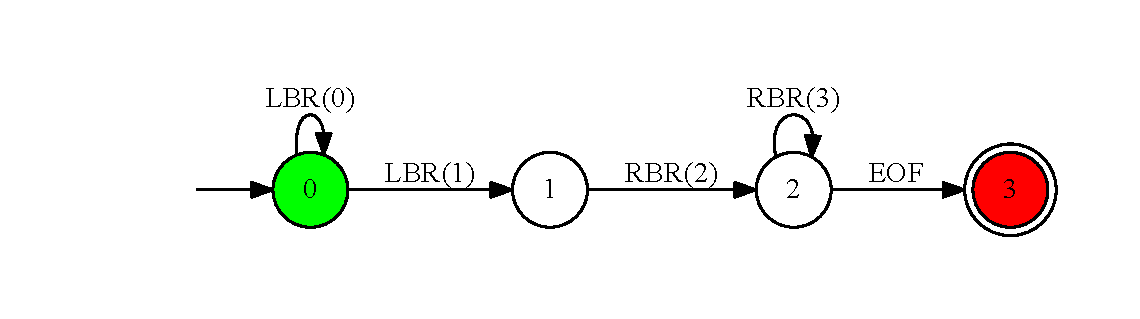
\includegraphics[width=170pt]{pictures/in3.pdf}
& \multirow{-10}*{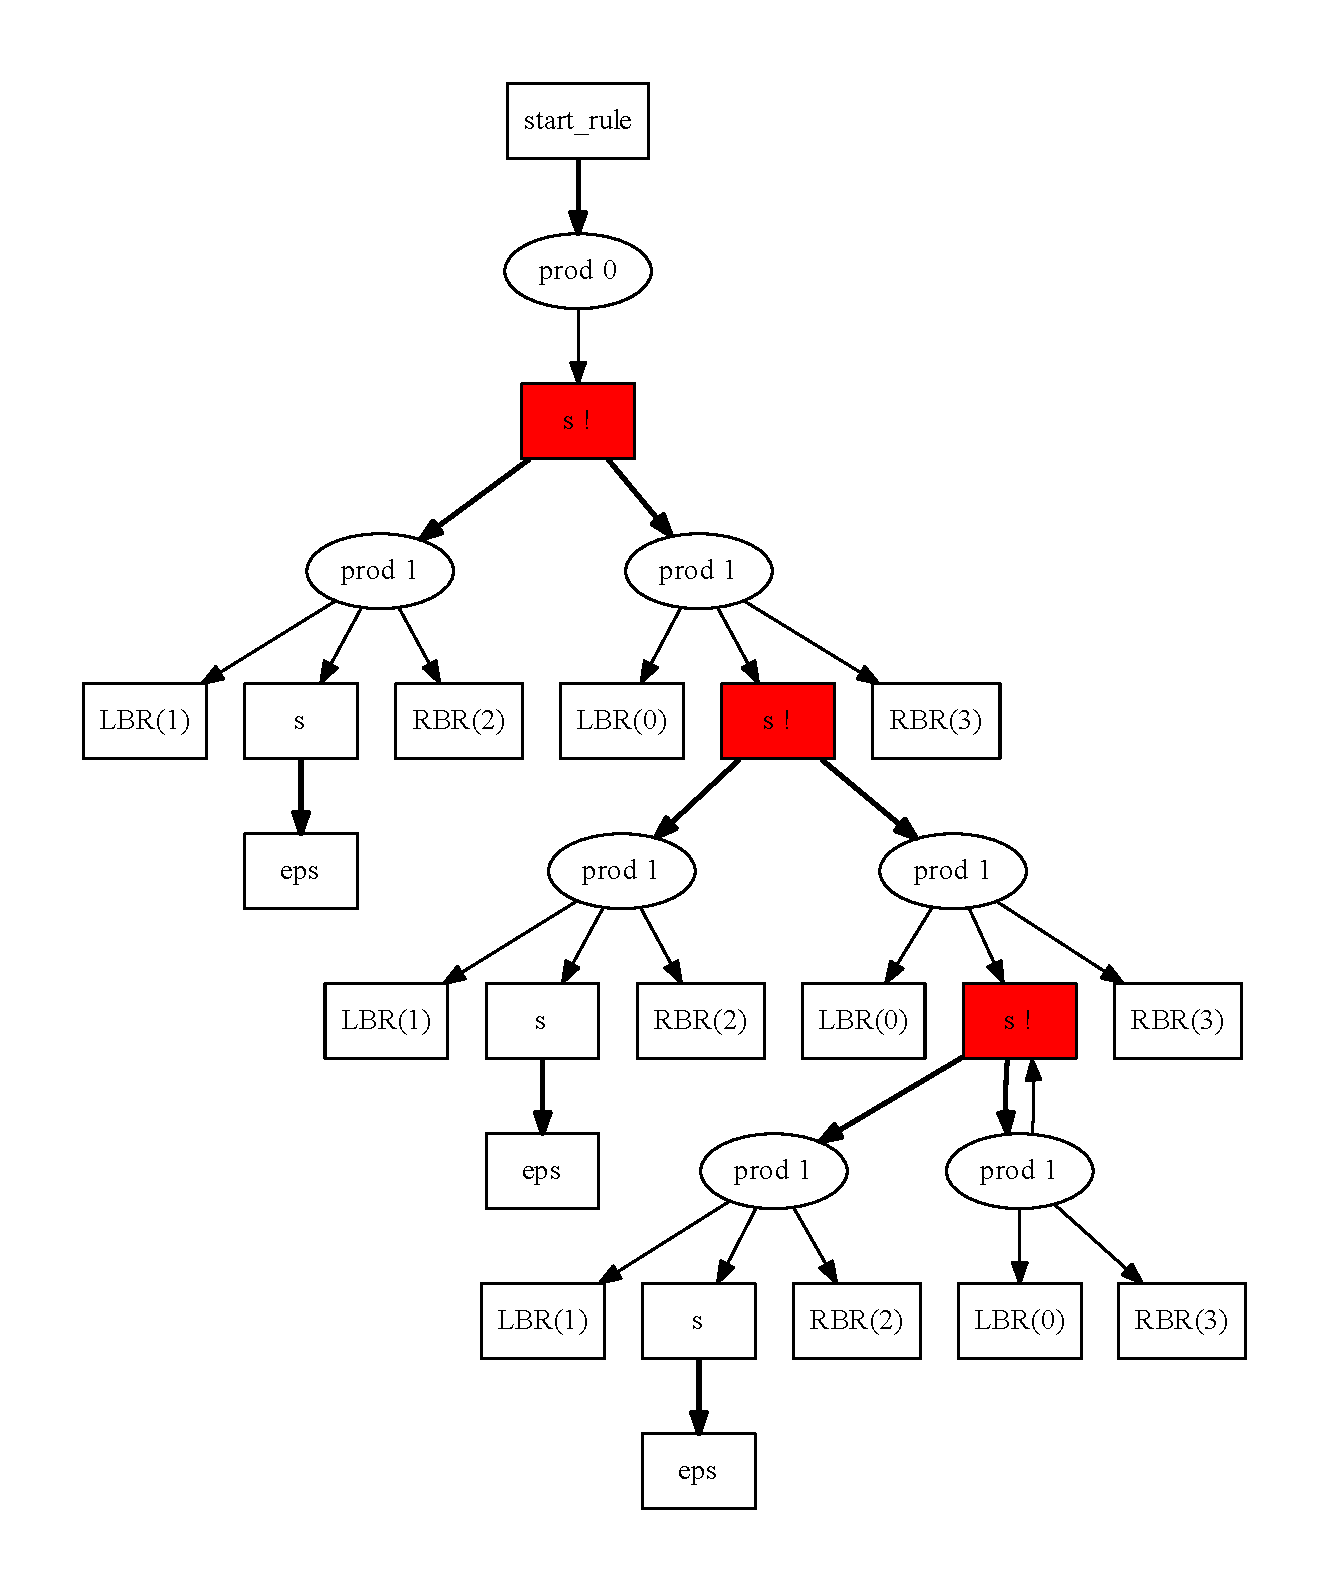
\includegraphics[width=170pt]{pictures/out3.pdf}}
\end{tabular}
\end{center}

\end{frame}

\begin{frame}[t]
    \transwipe[direction=90]
    \frametitle{Методология}
    \begin{itemize}
        \item  Берём и генерируем
    \end{itemize}
\end{frame}

\begin{frame}[t]
    \transwipe[direction=90]
    \frametitle{Апробация: замеры производительности}
    \begin{itemize}
        \item Подмножество T-SQL
        \item Входные КА эмулируют наиболее распростронённые типы входов
        \item ГРАФИКИ!!!
    \end{itemize}
\end{frame}

\begin{frame}[t]
    \transwipe[direction=90]
    \frametitle{Апробация: трансляция динамического SQL}
    \begin{itemize}
        \item Промышленный проект ООО ``Ланит-Терком'' по миграции ИС с MS-SQL Server на Oracle Server
        \item 850 хранимых процедур, 2,7 миллиона строк хранимого кода, более 3000 точек выполнения динамически формируемых запросов
        \item От 7 до 212 операторов для формирования одного запроса, 40 операторов в среднем
        \item Задача -- автоматизация трансляции динамически формируемых запросов
        \item Что-то про то, что автоматизация признана успешной
    \end{itemize}
\end{frame}

\begin{frame}[t]
    \transwipe[direction=90]
    \frametitle{Апробация: плагин к ReSharper}
    \begin{itemize}
        \item Поддержка встроенный языков в Microsoft Visual Studio IDE
        \begin{itemize}
            \item Поддержка встроенный языков в Microsoft Visual Studio IDE
            \begin{itemize}
                \item Подсветка синтаксиса
                \item Подсветка парных скобок
                \item ...
            \end{itemize}
        \end{itemize}
    \end{itemize}
\end{frame}

\begin{frame}
    \transwipe[direction=90]
    \frametitle{Публикации}
  \begin{itemize}
      \item Кириленко Я.А., Григорьев С. В., Авдюхин Д. А. Разработка синтаксических анализаторов в проектах по автоматизированному реинжинирингу информационных систем.  Научно-технические ведомости Санкт-Петербургского государственного политехнического университета информатика, телекоммуникации, управление. Т. 3, N 174, 2013. C. 94---98.
      \item Григорьев С. В., Вербицкая Е. А., Полубелова М. И., Иванов А. В., Мавчун Е. В. Инструментальная поддержка встроенных языков в интегрированных средах разработки. Моделирование и анализ информационных систем. Т. 21, N 6, 2014. С. 131---143.
      \item Григорьев С.В., Рагозина А.К. Обобщённый табличный LL-анализ. Системы и средства информатики. Т. 25, N 1, 2015. С. 89---107.
  \end{itemize} 
\end{frame}

\begin{frame}
    \transwipe[direction=90]
    \frametitle{Публикации}
  \begin{itemize}
          \item Semen Grigorev, Iakov Kirilenko. GLR-based abstract parsing. In Proceedings of the 9th Central \& Eastern European Software Engineering Conference in Russia (CEE-SECR ’13). 2013. ACM, New York, NY, USA. 1-9 p.
          \item Semen Grigorev, Ekaterina Verbitskaia, Andrei Ivanov, Marina Polubelova, Ekaterina Mavchun. String-embedded language support in integrated development environment. In Proceedings of the 10th Central and Eastern European Software Engineering Conference in Russia (CEE-SECR '14). 2014. ACM, New York, NY, USA. 1-11 p.
          \item Semen Grigorev, Iakov Kirilenko. From Abstract Parsing to Abstract Translation. Proceedings of the Spring/Summer Young Researchers' Colloquium on Software Engineering. 2014. Saint Petersburg, Russia. 1-5 p.
  \end{itemize} 
\end{frame}

\begin{frame}[fragile] 
    \transwipe[direction=90]
    \frametitle{Алгоритм: псевдокод}
\begin{algorithmic}[1]
\Function{parse}{$grammar, automaton$}
  \State{$inputGraph \gets$ construct inner graph representation of $automaton$}
  \State{$parserSource \gets$ generate RNGLR parser tables for $grammar$}
  \If{$inputGraph$ contains no edges}
    \If{$parserSource$ accepts empty input} {report success}
    \Else { report failure}
    \EndIf
  \Else
    \State{\Call{addVertex}{$inputGraph.startVertex, startState$}}
    \State{$\mathcal{Q}.Enqueue(inputGraph.startVertex)$}
    \While{$Q$ is not empty}
      \State{$v \gets \mathcal{Q}.Dequeue()$}
      \State{\Call{makeReductions}{$v$}}
      \State{\Call{push}{$v$}}
      \State{\Call{applyPassingReductions}{$v$}}
    \EndWhile
    \If{$v_f.level = q_f$ and $v_f.state$ is accepting} {report success}
    \Else { report failure}
    \EndIf
  \EndIf
\EndFunction
\end{algorithmic}
\end{frame}

\begin{frame}[fragile] 
    \transwipe[direction=90]
    \frametitle{Алгоритм: псевдокод}
\begin{algorithmic}[1]
%\caption{Single vertex processing}
%\label{processVertex}

\Function{makeReductions}{$innerGraphV$}
  \While{$innerGraphV.reductions$ is not empty}
    \State{$(startV, N, l) \gets innerGraphV.reductions.Dequeue()$}
    \State{find the set of vertices $\mathcal{X}$ reachable from $startV$}
    \State{    along the path of length ($l-1$), or $0$ if $l=0$;}
    \State{add $(startV, N, l-i)$ in $v.passingReductions$,}
    \State{    where $v$ is an $i$-th vertex of the path}
    \ForAll{$v_{h}$ in $\mathcal{X}$}
      \State{$state_{t} \gets$ calculate new state by $v_{h}.state$ and nonterminal $N$}
      \State{\Call{addEdge}{$v_{h}, startV, state_{t}, (l=0)$}}
    \EndFor
  \EndWhile
\EndFunction
\end{algorithmic}
\end{frame}


\begin{frame}[fragile] 
    \transwipe[direction=90]
    \frametitle{Алгоритм: псевдокод}
\begin{algorithmic}[1]

\Function{push}{$innerGraphV$}
  \State{$\mathcal{U} \gets$ copy $innerGraphV.unprocessed$}
  \State{clear $innerGraphV.unprocessed$}
  \ForAll{$v_{h}$ in $\mathcal{U}$}  
    \ForAll{$e$ in outgoing edges of $innerGraphV$}
      \State{$push \gets$ calculate next state by $v_{h}.state$ and the token on $e$}
      \State{\Call{addEdge}{$v_{h}, e.Head, push, false$}}
      \State{add $v_{h}$ in $innerGraphV.processed$}
    \EndFor
  \EndFor
\EndFunction

\Function{applyPassingReductions}{$innerGraphV$}
  \ForAll{$(v, edge)$ in $innerGraphV.passingReductionsToHandle$}
    \ForAll{$(startV, N, l) \gets v.passingReductions.Dequeue()$}
      \State{find the set of vertices $\mathcal{X}$,}
      \State{    reachable from $edge$ along the path of length ($l-1$)}
      \ForAll{$v_{h}$ in $\mathcal{X}$}
        \State{$state_{t} \gets$ calculate new state by $v_{h}.state$ and nonterminal $N$}
        \State{\Call{addEdge}{$v_{h}, startV, state_{t}, false$}}
      \EndFor
    \EndFor
  \EndFor
\EndFunction
\end{algorithmic}
\end{frame}

\begin{frame}[fragile] 
    \transwipe[direction=90]
    \frametitle{Алгоритм: псевдокод}
\begin{algorithmic}[1]
%\caption{GSS construction}
%\label{gss_construction}
\Function{addVertex}{$innerGraphV, state$}
  \State{$v \gets$ find a vertex with state $=state$ in}
  \State{    $innerGraphV.processed \cup innerGraphV.unprocessed$}
  \If{$v$ is not $null$ } \Comment{The vertex have been found in GSS}
    \State{\Return{($v, false$)}} 
  \Else
    \State{$v \gets$ create new vertex for $innerGraphV$ with state $state$}
    \State{add $v$ in $innerGraphV.unprocessed$}
    \ForAll{$e$ in outgoing edges of $innerGraphV$}
      \State{calculate the set of zero-reductions by $v$}
      \State{    and the token on $e$ and add them in $innerGraphV.reductions$}
    \EndFor
    \State{\Return{$(v, true$)}}
  \EndIf
\EndFunction
\end{algorithmic}
\end{frame}

\begin{frame}[fragile] 
    \transwipe[direction=90]
    \frametitle{Алгоритм: псевдокод}
\begin{algorithmic}[1]
\Function{addEdge}{$v_{h}, innerGraphV, state_{t}, isZeroReduction$}
  \State{$(v_{t}, isNew) \gets$ \Call{addVertex}{$innerGraphV, state_{t}$}}
  \If{GSS does not contain edge from $v_{t}$ to $v_{h}$}
    \State{$edge \gets$ create new edge from $v_{t}$ to $v_{h}$}
    \State{$\mathcal{Q}.Enqueue(innerGraphV)$}
    \If{not $isNew$ and $v_{t}.passingReductions.Count>0$}
      \State{add $(v_{t}, edge)$ in $innerGraphV.passingReductionsToHandle$}
    \EndIf
    \If{not $isZeroReduction$}
      \ForAll{$e$ in outgoing edges of $innerGraphV$}
        \State{calculate the set of reductions by $v$}
        \State{    and the token on $e$ and add them in $innerGraphV.reductions$}
      \EndFor
    \EndIf
  \EndIf
\EndFunction
\end{algorithmic}
\end{frame}



\end{document}
